%#! platex main.tex

%======================================================================
\chapter{提案手法}

本章では, ワイヤレスイヤホンに搭載されたマイクを使用して, 録音した食事中の音から食品認識と咀嚼検出を行う手法について詳述する. 咀嚼音には食材の硬さや質感, 噛むタイミングなどの情報が含まれていると考える. 例えば, ポテトチップスの咀嚼音は特有であり, その音を聞くだけでポテトチップスであると認識し, 咀嚼のタイミングを推測することが可能である.

食事中の音には, 咀嚼音の他に, 皿や箸などのカトラリによる音や環境ノイズも含まれている. 食品認識や咀嚼検出を高い精度で行うためには, これらのノイズを減らし, 咀嚼音のみを効果的に抽出することが重要なステップとなる. この点で, ワイヤレスイヤホンは耳に装着され, 咀嚼音が発生する口に近い位置にあるため, 咀嚼音の要素を多く含んだ音を記録することに優位性を持つ.

食品認識では, 食事中の音データを0.5秒のセグメントに分割し, これらのセグメントをメルスペクトログラムに変換し, 畳み込みニューラルネットワーク(CNN)での学習を通じて食品認識モデルを生成する. 咀嚼検出についても同様のアプローチをとり, セグメントをメルスペクトログラムに変換し, CNNで学習を行い, 咀嚼検出モデルを生成する. 咀嚼検出における正解ラベルは, セグメント内に咀嚼タイムスタンプが1つ以上存在する場合を「咀嚼あり」, 存在しない場合を「咀嚼なし」とする.

学習に使用するデータセットは, 前章で説明したデータ収集アプリケーションによって収集されたデータを使用する. このデータセットには, 食事中の音データと正解データが含まれる. ただし, 食事中の音データは1ファイル1品のみであり, 正解データには食品の種類と咀嚼タイムスタンプが含まれる. 図\ref{fig:wave-sample}にポテトチップスのデータの例を示す. これらのデータを用いて, 精度の高い食品認識と咀嚼検出モデルの構築を目指す.

\begin{figure}[t]
    \begin{center}
        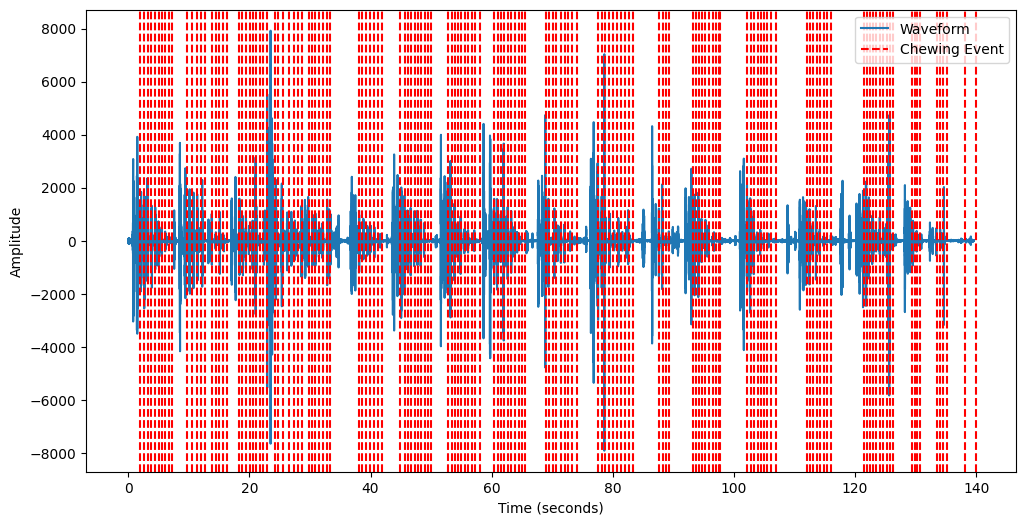
\includegraphics[clip,  width=0.95\hsize]{img/wave-sample.png}
        \caption{データ収集アプリケーションによって収集されたデータの例}
        \label{fig:wave-sample}
    \end{center}
\end{figure}

\begin{figure*}[t]
    \centering

    \begin{minipage}[b]{0.3\hsize}
        \centering
        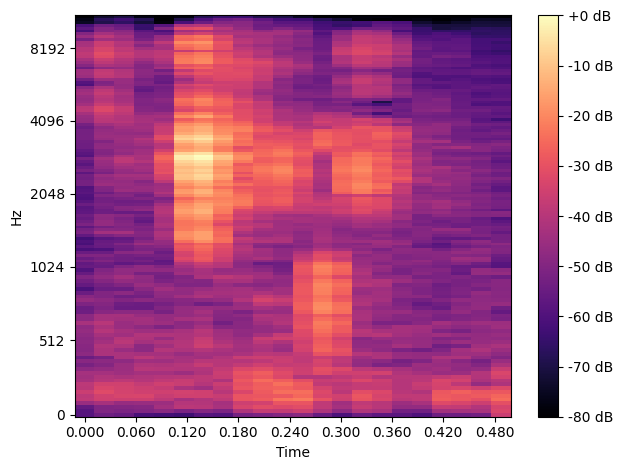
\includegraphics[width=\hsize]{img/melspec/rice.png}
        \subcaption{ご飯}
    \end{minipage}
    \begin{minipage}[b]{0.3\hsize}
        \centering
        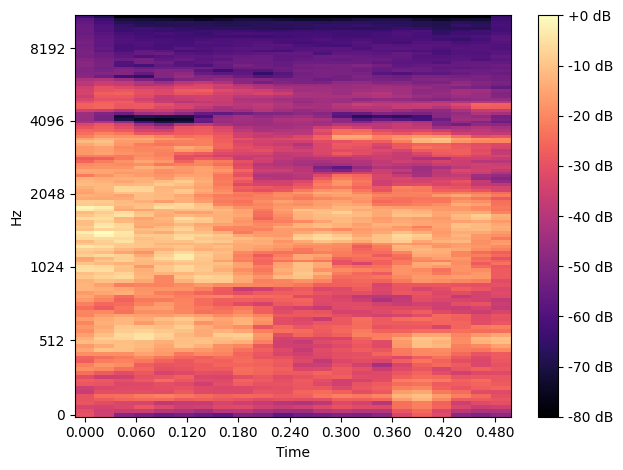
\includegraphics[width=\hsize]{img/melspec/soup.png}
        \subcaption{味噌汁}
    \end{minipage}
    \begin{minipage}[b]{0.3\hsize}
        \centering
        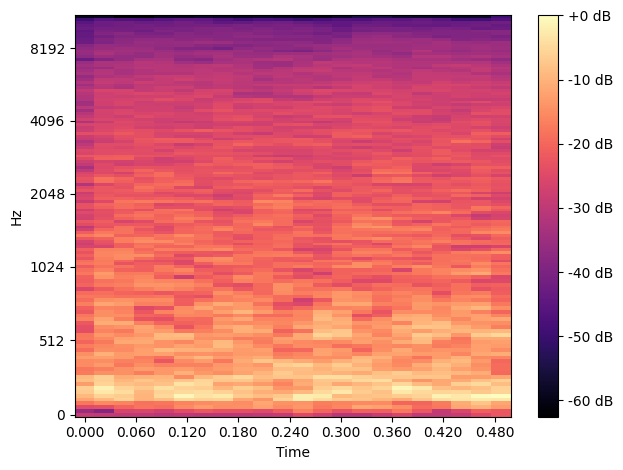
\includegraphics[width=\hsize]{img/melspec/salad.png}
        \subcaption{サラダ}
    \end{minipage}

    \hspace{0.3cm}

    \begin{minipage}[b]{0.3\hsize}
        \centering
        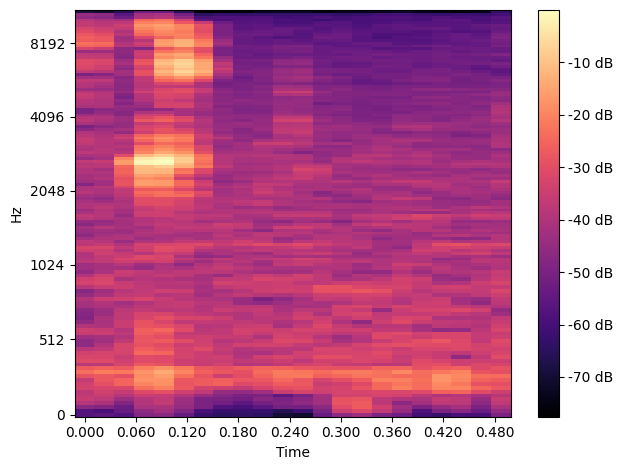
\includegraphics[width=\hsize]{img/melspec/rice-cookie.png}
        \subcaption{せんべい}
    \end{minipage}
    \begin{minipage}[b]{0.3\hsize}
        \centering
        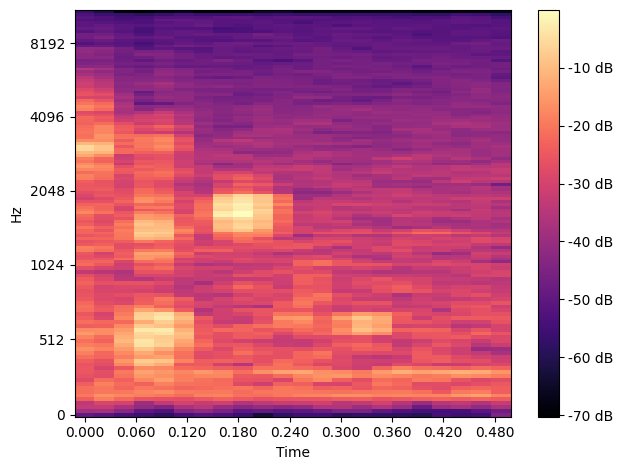
\includegraphics[width=\hsize]{img/melspec/potato-chips.png}
        \subcaption{ポテトチップス}
    \end{minipage}
    \begin{minipage}[b]{0.3\hsize}
        \centering
        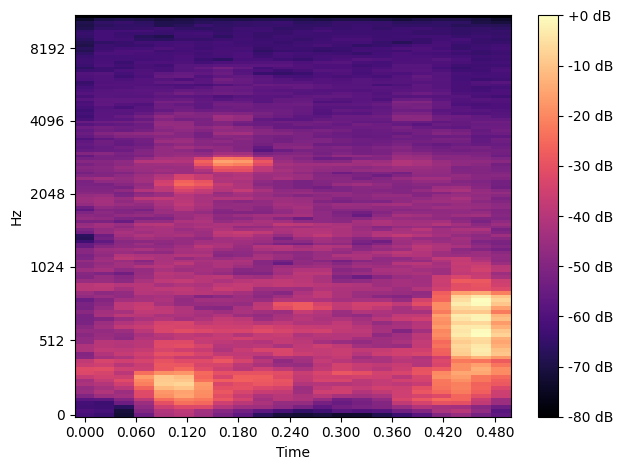
\includegraphics[width=\hsize]{img/melspec/yakisoba.png}
        \subcaption{焼きそば}
    \end{minipage}

    \caption{食品別のメルスペクトログラムの一例}
    \label{fig:sample-melspec-data}
\end{figure*}

%----------------------------------------------------------------------
\section{食品認識}

本稿では, 畳み込みニューラルネットワーク(CNN)とリカレントニューラルネットワーク(RNN)を基盤とし, 食事中の音データから変換されたメルスペクトログラムを学習データとして活用し, 食品認識モデルの構築を行う. メルスペクトログラムを用いてCNNで音声分類を行うと従来の手法よりも精度が出ることが言われているため\cite{Dossou_2021_ICCV}, 本研究でもこの手法を採用する. メルスペクトログラムは, 音声信号の特徴を表現するために広く用いられる視覚的表現であり, 人間の可聴領域に基づくメル尺度によるスペクトログラムの一種である. 食品別のメルスペクトログラムの一例を図\ref{fig:sample-melspec-data}に示す. 咀嚼音は可聴領域に多く含まれており, メルスペクトログラムはこれらの特徴を効率的に捉えることが可能であると考えている. さらに, CNNだけでなくRNNとの組み合わせにより, メルスペクトログラムの空間的特徴だけでなく, 音データの時間的特徴も捉えることができる.

学習データセットの構築に関しては, まず音データを$22050Hz$にリサンプリングし, $500Hz$以下と$5000Hz$以上の周波数帯を削除するために, 音データに対してローパスフィルタとハイパスフィルタを適用する. 次に, 音データをウィンドウ幅$500ms$, オーバーラップ率$0.75$のスライディングウィンドウで部分時系列データに分割する. ただし, 部分時系列データの長さを統一するため, $500ms$以下のデータは除外する. さらに, 部分時系列データ中に手動による咀嚼タイムスタンプが含まれず, 最大信号強度が$-40dBFS$に満たないものは食品ラベルを含まないものとして扱う. 最後に, 部分時系列データは特徴抽出のために, FFTのウィンドウサイズが$1024$, フレーム間のホップ長が$256$, メルバンドの数が$64$のメルスペクトログラムに変換する. これらのデータを訓練データ$90\%$とテストデータ$10\%$に分割し, 訓練データを用いてCNNとRNNのハイブリッドモデルで学習させる. CNNには3つの畳み込み層を使用し, それぞれの畳み込み層の後に正規化層とプーリング層を適用する. さらにこれらの出力をフラット化し, RNN層に入力する. RNNの出力から最後の隠れ層を取り出し, 過学習を防ぐためにドロップアウト層を適用する. 最後に全結合層でRNNの出力を最終的な食品のクラス数に対応する出力に変換する. 学習後のモデルの精度評価については, テストデータを用いて, 混同行列を算出し, 精度, 再現率, F値を算出する.


%----------------------------------------------------------------------
\section{咀嚼検出}

咀嚼検出においても, 食品認識と同様CNNとRNNを組み合わせたモデルを使用する. 学習データセットに関しても食品認識と同様にリサンプリング・フィルタリングを施し, スライディングウィンドウにより部分時系列データに分割する. さらに, 部分時系列データ中に手動による咀嚼タイムスタンプが含まれているかどうかを確認し, 含まれている場合は「咀嚼あり」, 含まれていない場合は「咀嚼なし」というラベルを付与する. ただし, 手動による咀嚼タイムスタンプは押すタイミングによる誤差が発生するので, 前後$500ms$に範囲を広げて咀嚼タイムスタンプの有無を確認する. これらのデータを訓練データ$90\%$とテストデータ$10\%$に分割し, 訓練データを用いてCNNとRNNのハイブリッドモデルで学習させる. CNNには3つの畳み込み層を使用し, それぞれの畳み込み層の後に正規化層とプーリング層を適用する. さらにこれらの出力をフラット化し, RNN層に入力する. RNNの出力から最後の隠れ層を取り出し, 過学習を防ぐためにドロップアウト層を適用する. 最後に全結合層でRNNの出力を咀嚼の有無に変換する. 学習後のモデルの精度評価については, テストデータを用いて, 混同行列を算出し, 精度, 再現率, F値を算出する.

% 以下はRefTeX用
%%% Local Variables:
%%% mode: yatex
%%% TeX-master: "main"
%%% End:
